% Source for the figure of IntervalTree (sec. 16.4): seven intervals in the
% map ordered by (a, b), each node with its interval (left) and the largest
% right end of its subtree (right); above, the nodes that stabbed(7) visits
% (shaded); below, the tree after insert(3, 13), the new node and the
% augmented values that the joins recompute shaded. Build: make figures (in
% ../build).
\documentclass[border=4pt]{standalone}
\usepackage[T1]{fontenc}
\usepackage{newpxtext,newpxmath}
\usepackage[varqu,varl,scaled=0.95]{zi4}
\usepackage{tikz}
% tikz-ads.tex: the TikZ styles shared by the figures of the memory of the
% manual, \input by each standalone figure: a cell of a vector (cell), the
% cell that an operation touches (touched), a free cell (free), a node of a
% linked structure (node), the labels of indices (index) and of variables
% (var), a pointer (ptr), and \cells and \indices to draw a row of cells.
\usetikzlibrary{arrows.meta,positioning,calc,fit,shapes.multipart}
\definecolor{adsTouched}{RGB}{214,196,236}
\definecolor{adsFree}{RGB}{236,236,236}
\tikzset{
  ads/.style={>={Stealth[length=2mm]},font=\small,
              every node/.append style={inner sep=0pt}},
  cell/.style={draw,minimum width=7mm,minimum height=7mm,
               font=\small\ttfamily,outer sep=0pt},
  touched/.style={cell,fill=adsTouched},
  free/.style={cell,fill=adsFree,text=black!45},
  node/.style={draw,rounded corners=1pt,minimum width=8mm,
               minimum height=6mm,font=\small\ttfamily},
  index/.style={font=\scriptsize\ttfamily,text=black!60},
  var/.style={font=\small\itshape},
  ptr/.style={->,thick}
}
% \cells{name}{x,y}{list}: a row of cells, the first at (x,y), named
% name-0, name-1, ...; each item is text/style, the style one of cell,
% touched and free (e.g., {a/cell,e/touched,/free})
\newcommand{\cells}[3]{%
  \foreach \v/\s [count=\i from 0] in {#3}
    \node[\s] (#1-\i) at ($(#2)+(\i*7mm,0)$) {\v};}
% \indices{name}{n}: the indices 0 .. n-1 under the cells of name
\newcommand{\indices}[2]{%
  \foreach \i in {0,...,\numexpr#2-1\relax}
    \node[index,below=1.2mm of #1-\i] {\i};}

\tikzset{
  iv/.style={rectangle split,rectangle split parts=2,
             rectangle split horizontal,draw,font=\small\ttfamily,
             inner xsep=1.5mm,inner ysep=1.2mm},
  ivt/.style={iv,rectangle split part fill={adsTouched,adsTouched}},
  ivh/.style={iv,rectangle split part fill={white,adsTouched}},
  edge/.style={thick}
}
% \ivn{name}{style}{x,y}{interval}{aug}
\newcommand{\ivn}[5]{\node[#2] (#1) at (#3)
  {#4\nodepart{two}#5};}
\begin{document}
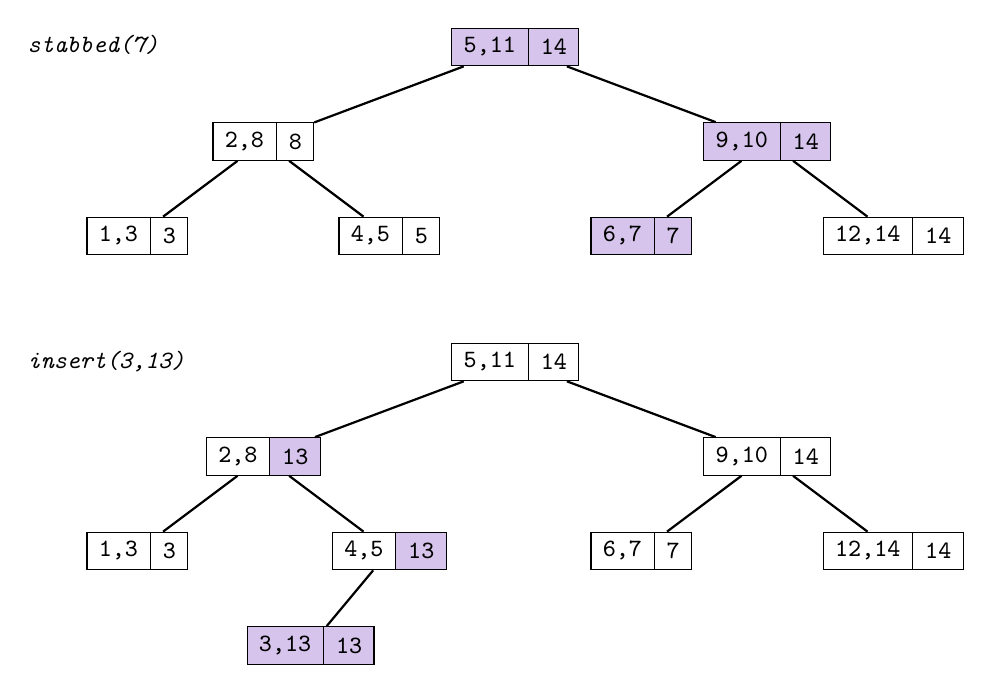
\begin{tikzpicture}[ads]
  % before: stabbed(7) goes right at [5,11], left at [9,10], right at [6,7]
  \node[var,anchor=west] at (-62mm,0) {\texttt{stabbed(7)}};
  \ivn{r}{ivt}{0,0}{5,11}{14}
  \ivn{l}{iv}{-32mm,-12mm}{2,8}{8}
  \ivn{rr}{ivt}{32mm,-12mm}{9,10}{14}
  \ivn{ll}{iv}{-48mm,-24mm}{1,3}{3}
  \ivn{lr}{iv}{-16mm,-24mm}{4,5}{5}
  \ivn{rl}{ivt}{16mm,-24mm}{6,7}{7}
  \ivn{rrr}{iv}{48mm,-24mm}{12,14}{14}
  \draw[edge] (r) -- (l); \draw[edge] (r) -- (rr);
  \draw[edge] (l) -- (ll); \draw[edge] (l) -- (lr);
  \draw[edge] (rr) -- (rl); \draw[edge] (rr) -- (rrr);
  % after insert(3,13): a new leaf under [4,5]
  \begin{scope}[yshift=-40mm]
  \node[var,anchor=west] at (-62mm,0) {\texttt{insert(3,13)}};
  \ivn{r}{iv}{0,0}{5,11}{14}
  \ivn{l}{ivh}{-32mm,-12mm}{2,8}{13}
  \ivn{rr}{iv}{32mm,-12mm}{9,10}{14}
  \ivn{ll}{iv}{-48mm,-24mm}{1,3}{3}
  \ivn{lr}{ivh}{-16mm,-24mm}{4,5}{13}
  \ivn{rl}{iv}{16mm,-24mm}{6,7}{7}
  \ivn{rrr}{iv}{48mm,-24mm}{12,14}{14}
  \ivn{n}{ivt}{-26mm,-36mm}{3,13}{13}
  \draw[edge] (r) -- (l); \draw[edge] (r) -- (rr);
  \draw[edge] (l) -- (ll); \draw[edge] (l) -- (lr);
  \draw[edge] (rr) -- (rl); \draw[edge] (rr) -- (rrr);
  \draw[edge] (lr) -- (n);
  \end{scope}
\end{tikzpicture}
\end{document}
